%% ==============================
%\chapter{Appendix}
%\label{ch:Appendix}
%% ==============================

\appendix
\addchap{Appendix}

\section{Method}
\label{app:treatment}
\begin{lstlisting}[language=bash,caption={Bash script details for the treatment of the Fermi LAT data.},label={app:script}, breaklines=true]
#First, install the Fermi science tools from: https://fermi.gsfc.nasa.gov/ssc/data/analysis/software/
#All I'm saying here is better explained in analysis thread: https://fermi.gsfc.nasa.gov/ssc/data/analysis/scitools/ You can look at the following threads: Extract LAT Data, Using LAT All-sky Weekly Files, (Un)Binned Likelihood Tutorial
#Also every command has a documentation at this address: https://fermi.gsfc.nasa.gov/ssc/data/analysis/scitools/help/<name of the command>.txt
fileBase="Base_name_of_all_files_produced_in_this_run"
spacecraft="location_of_the_spacecraft_file_containing_positions_and_infos_about_the_satellite"
#Some numbers that are used multiple times:
number_of_pixels_in_lon=720
number_of_pixels_in_lat=360
pixel_size=0.5

#Select the events from the weekly files listed in file_list.txt. (ra, dec) is the galactic center coordinates in ICRS system, a radius of 180 to select the whole sky, and the energy bounds. The one here correspond to the energy bound of the Fermi diffuse model. You might run into troubles later if you try to use it with energies out of this range
gtselect evclass = 256 
	evtype = 3 \
	infile = file_list.txt \
	outfile = $fileBase.fits \
	ra = 266.4049882865447 \
	dec = -28.93617776179147 \
	rad = 180 \
	tmin = INDEF \
	tmax = INDEF \
	emin = 58.4731 \
	emax = 513056 \
	zmax = 90
#Disregard all events registered out of the Good Time Intervals of the spacecraft, with the cut recommended by Fermi peoples
gtmktime scfile = $spacecraft \
	filter = "DATA_QUAL>0 && LAT_CONFIG==1 && ABS(ROCK_ANGLE)<52" \
	roicut = no \
	evfile = $fileBase".fits" \
	outfile = $fileBase"_gtmktime.fits"
#Making the first map from the events. All options are on the web. The settings of this map are reused later for the exposure for example.
gtbin algorithm = "CCUBE" \
	evfile = $fileBase"_gtmktime.fits" \
	outfile = $fileBase"_ccube.fits" \
	scfile = $spacecraft \
	nxpix = $number_of_pixels_in_lon \
	nypix = $number_of_pixels_in_lat \
	binsz = $pixel_size \
	coordsys = GAL \
	xref = $l \
	yref = $b \
	axisrot = 0 \
	proj = "CAR" \
	ebinalg = "LOG" \
	emin = 59 \
	emax = 513000 \
	enumbins = 30
#Make a first exposure map with default settings. It can take a long time. Here the zmax=90 is to avoid the earth limbs contamination.
gtltcube zmax = 90 \
	evfile = $fileBase"_gtmktime.fits" \
	scfile = $spacecraft \
	outfile = $fileBase"_ltcube.fits" \
	dcostheta = 0.025 \
	binsz = 1
#Bin the exposure map in the same binning than gtbin. The only difference is for the energy bins: It creates a map for every energy bin's "EDGE" when gtbin creates a map for every energy bin's "CENTER". This can be changed via "bincalc" option but you need to let it on edge for later.
#You can also do once a full exposure map, even if you analyze only a small sky region, if you don't change the cuts in gtselect you can then reuse it.
gtexpcube2 bincalc="EDGE" \
	infile = $fileBase"_ltcube.fits" \
	cmap = $fileBase"_ccube.fits" \
	outfile = $fileBase"_expcube.fits" \
	irfs = "CALDB" \
	nxpix = $number_of_pixels_in_lon \
	nypix = $number_of_pixels_in_lat \
	binsz = $pixel_size \
	xref = 0. \
	yref = 0. \
	axisrot = 0 \
	proj = "CAR" \
	coordsys = GAL \
	ebinalg = "LOG" \
	emin = 59 \
	emax = 513000 \
	enumbins = 30
#Now you can divide your gtbin map by your gtexpcube2 map to get a flux map! Use this:
ftpixcalc outfile = $fileBase"_flux.fits" \
    expr = a/b \
    a = $fileBase"_ccube.fits" \
    b = $fileBase"_expcube.fits"
#Now to subtract the point sources:
#Let allow energy dispersion now, it is better too soon than too late.
export USE_BL_EDISP=true
#Create an .xml file that lists all the point sources or diffuse sources you want to add to your model. Here I add all the point sources that could play a role in my maps (it knows it from the gtmktime file), but also the diffuse Fermi background (gll_iem_v06.fits) and the Fermi isotropic template (iso_P8R2_CLEAN_V6_v06.txt). You will have to comment them out by hand afterward in the $fileBase"_model.xml" file if you don't want them in your model. The point sources are taken from the 3FGL catalog (gll_psc_v16.fit), for a significance > 3.
python make3FGLxml.py gll_psc_v16.fit $fileBase"_gtmktime.fits" \
    -o $fileBase"_model.xml" \
    -G $FERMI_DIR/refdata/fermi/galdiffuse/gll_iem_v06.fits \
    -g gll_iem_v06 \
    -I $FERMI_DIR/refdata/fermi/galdiffuse/iso_P8R2_CLEAN_V6_v06.txt \
    -i iso_P8R2_CLEAN_V6_v06 \
    --extDir=$storage_path/processing/ \
    -s 3.
#This will create a map of each source listed in your .xml file with the same parameters than your gtbin map. You have to do it at least once for the diffuse sources, but point sources are done quickly and can be done later (via option ptsrc = yes/no). This can take some time and the output file is quickly very big with the point sources.
gtsrcmaps scfile = $spacecraft \
    expcube = $fileBase"_ltcube.fits" \
    cmap = $fileBase"_ccube.fits" \
    srcmdl = $fileBase"_model.xml" \
    bexpmap = $fileBase"_expcube.fits" \
    outfile = $fileBase"_srccube.fits" \
    irfs = CALDB
#This OPTIONAL step is here to fit every point sources to your data to try to improve the 3FGL catalog and subtract a better model. You obviously need all backgrounds from fermi, iso template point and diffuse sources. This will create a new improved .xml file with slightly different values for every point sources than the one created by make3FGLxml.py. This take A LOT of time for big regions and can not be done for the whole sky at once. If you want to do it you need to cut the sky in smaller regions and reassemble them again after. That might not be worth it...
gtlike refit = no \
	plot = no \
	sfile = $fileBase"_gtlike.xml" \
	statistic = BINNED \
	cmap = $fileBase"_srccube.fits" \
	bexpmap = $fileBase"_expcube.fits" \
	expcube =  $fileBase"_ltcube.fits" \
	srcmdl =  $fileBase"_model.xml" \
	irfs = CALDB \
	optimizer = NEWMINUIT
#You can finally create a model map of the sources to subtract. The point sources are calculated automatically if they are not found in the gtsrcmaps file.
gtmodel srcmaps = $fileBase"_srccube.fits" \
	srcmdl = $fileBase"_model.xml" \
	outfile =  $fileBase"_modelcube_ptsrc.fits" \
	irfs = CALDB \
	expcube = $fileBase"_ltcube.fits" \
	bexpmap = $fileBase"_expcube.fits" \
	outtype = CCUBE
#You can finally subtract the gtmodel map from your gtbin map via:
ftpixcalc outfile = $fileBase"_diffuse.fits" \
    expr = a-b \
    a = $fileBase"_ccube.fits" \
    b = $fileBase"_modelcube_ptsrc.fits"  
\end{lstlisting}


\newpage
\begin{figure}[H]
  \centering
  \begin{minipage}[h]{0.45\textwidth}
  	\centering
	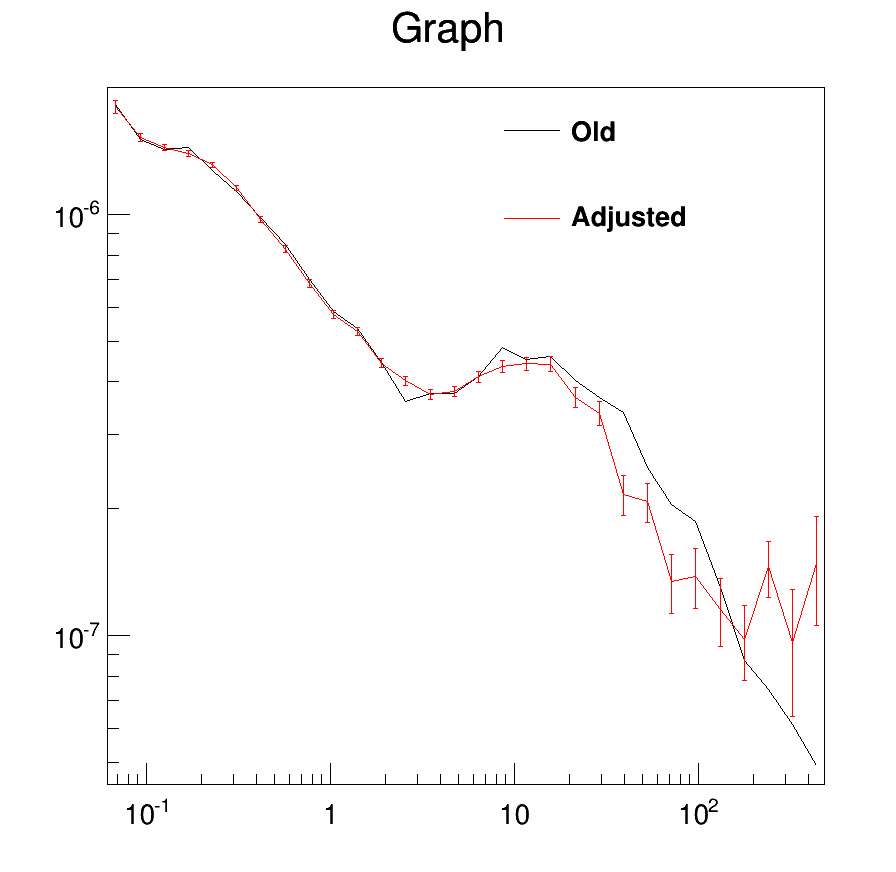
\includegraphics[width=1.\linewidth]{pic/method/app_iso_process_1.png}
  	\subcaption{}
  	\label{app:app_iso_process_1}
  \end{minipage}
  \hfill
  \begin{minipage}[h]{0.45\textwidth}
  	\centering
	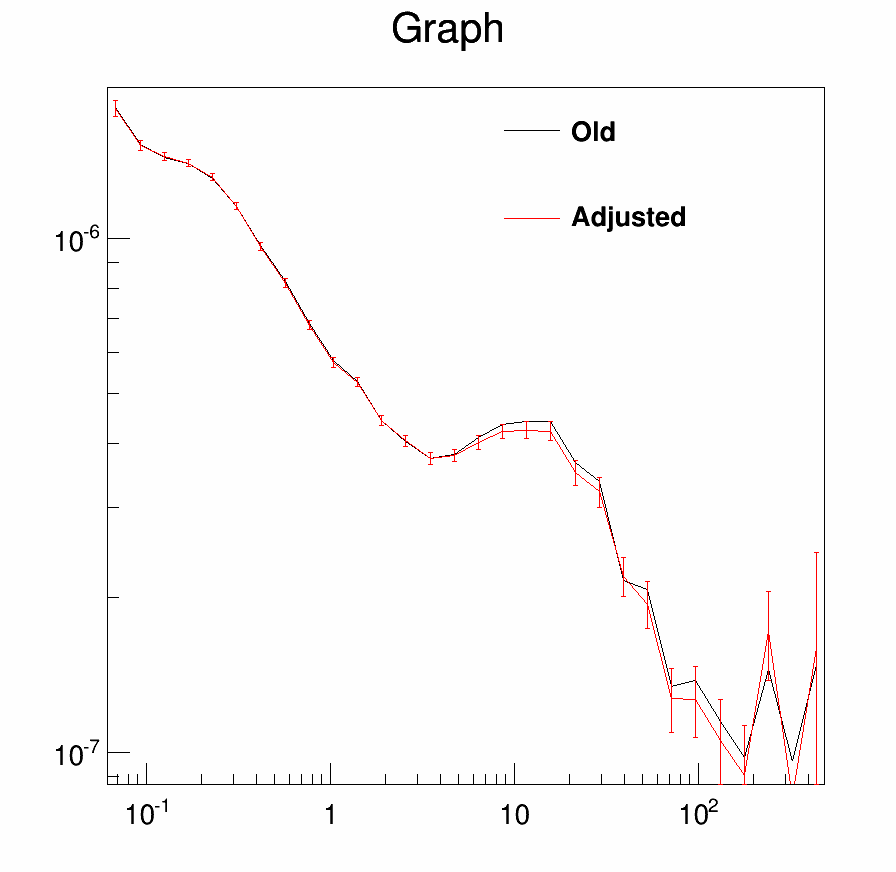
\includegraphics[width=1.\linewidth]{pic/method/app_iso_process_2.png}
  	\subcaption{}
  	\label{app:app_iso_process_2}
  \end{minipage}
  \hfill
  \begin{minipage}[h]{0.45\textwidth}
  	\centering
	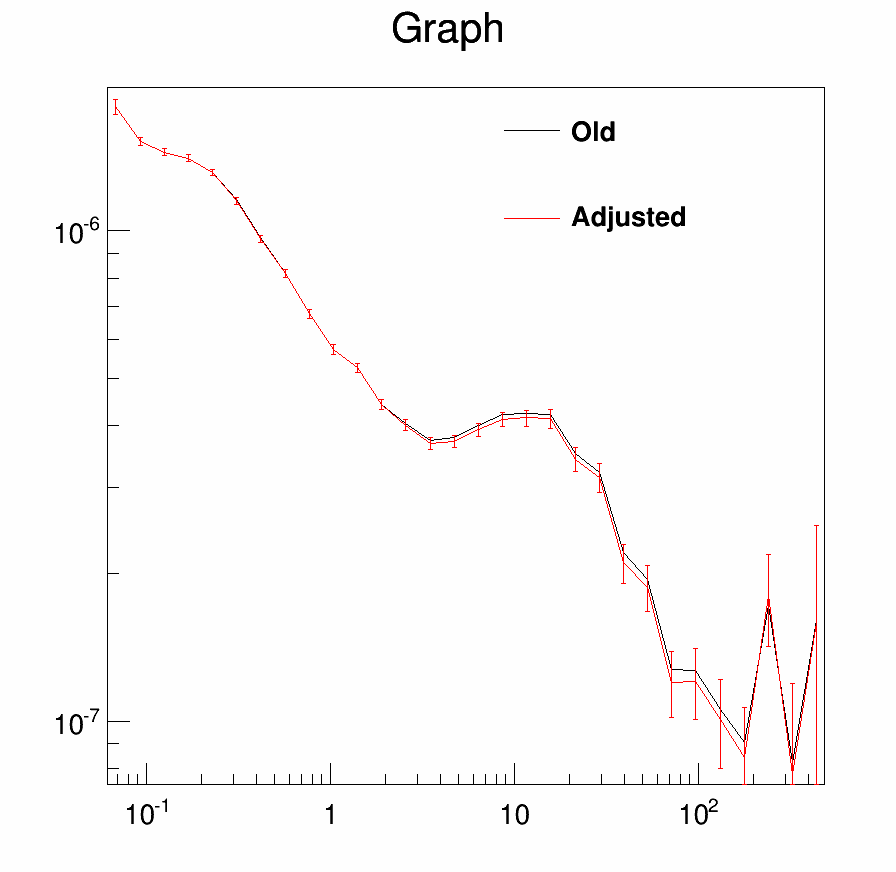
\includegraphics[width=1\linewidth]{pic/method/app_iso_process_3.png}
 	\subcaption{}
  	\label{app:app_iso_process_3}
  \end{minipage}
  \hfill
  \begin{minipage}[h]{0.45\textwidth}
  	\centering
	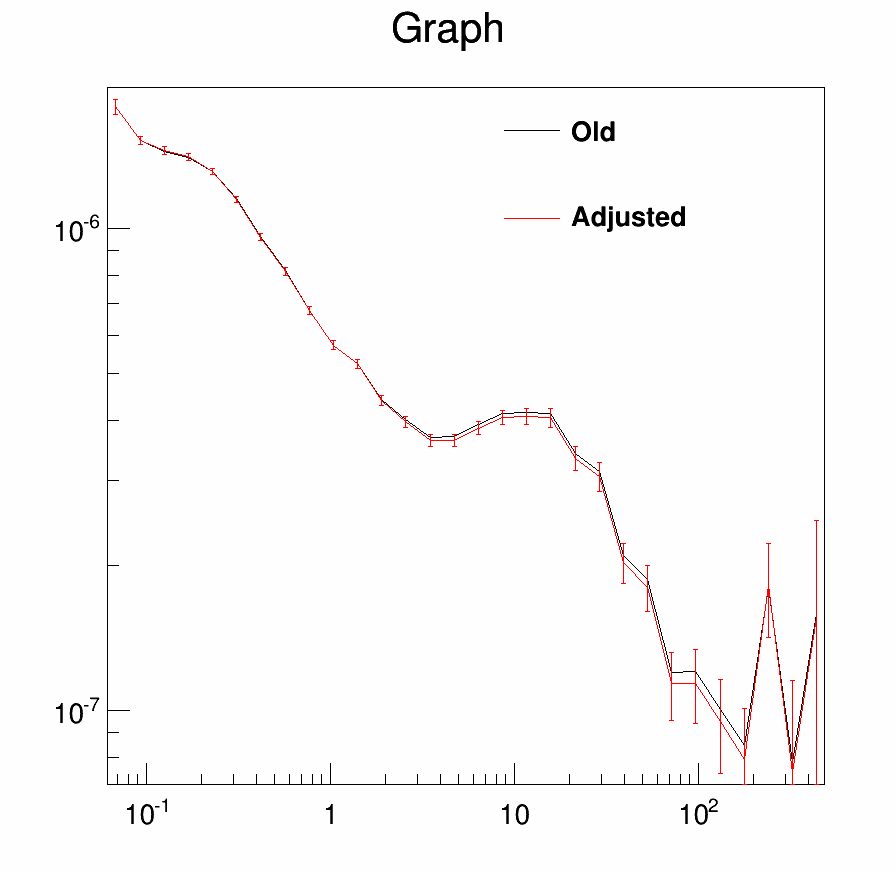
\includegraphics[width=1\linewidth]{pic/method/app_iso_process_4.png}
  	\subcaption{}
  	\label{app:app_iso_process_4}
  \end{minipage}
  \caption[Isotropic template convergence.]{Isotropic recalibration process. Each graph compares the precedent (in black) and the new (in red) isotropic template. The initial template is the Fermi template iso\char`_P8R2\char`_CLEAN\char`_V6\char`_v06 that is given with the Fermi tools \cite{FermiTools}. The convergence is reached after a few steps, even if high energies continue to fluctuate longer due to higher uncertainties.}
  \label{app:app_iso_process}
\end{figure}





\newpage
\section{First results: Study of the excess}
\label{app:BKG_distributions}
\begin{figure}[H]
  \centering
  \begin{minipage}[h]{0.45\textwidth}
  	\centering
	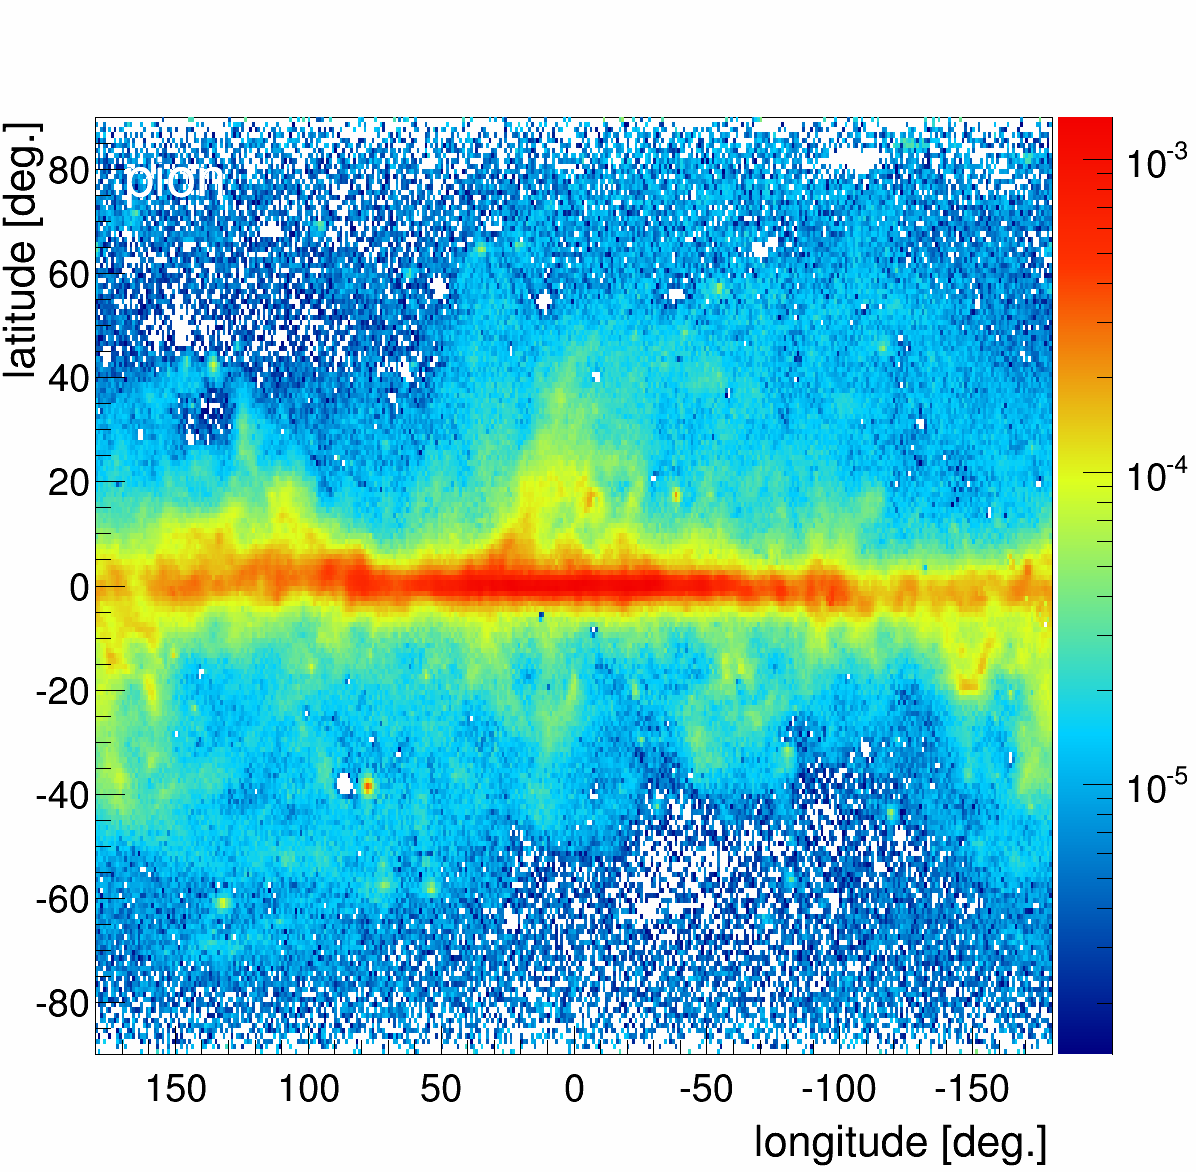
\includegraphics[width=1.\linewidth]{pic/results/BKG_PCR_Integral.png}
  	\subcaption{}
  	\label{app:BKGonly_PCR}
  \end{minipage}
  \hfill
  \begin{minipage}[h]{0.45\textwidth}
  	\centering
	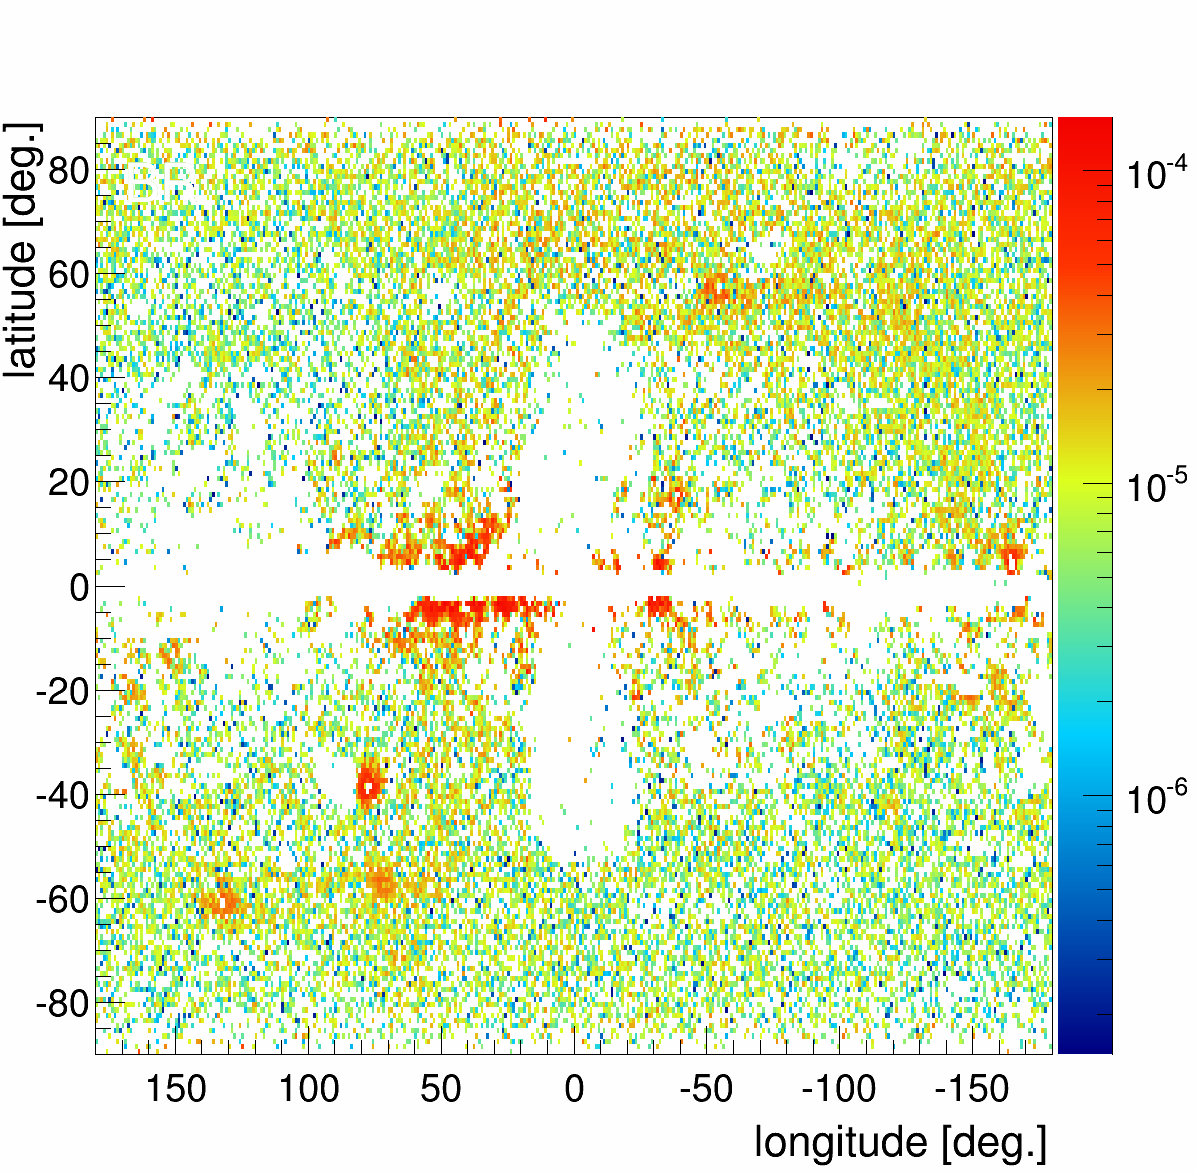
\includegraphics[width=1.\linewidth]{pic/results/BKG_BR_Integral.png}
  	\subcaption{}
  	\label{app:BKGonly_BR}
  \end{minipage}
  \hfill
  \begin{minipage}[h]{0.45\textwidth}
  	\centering
	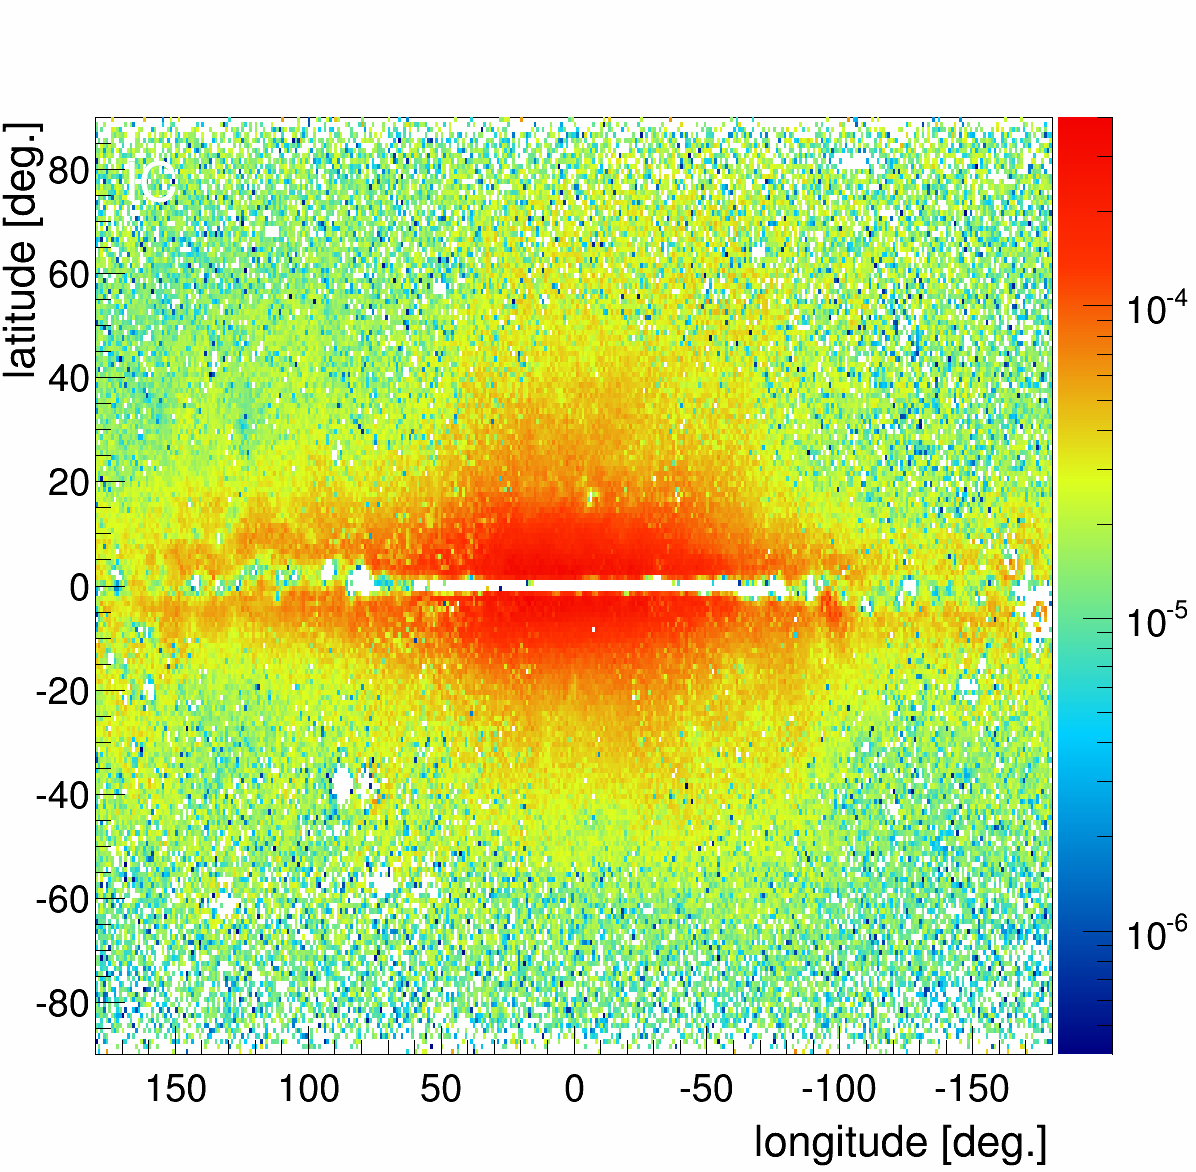
\includegraphics[width=1\linewidth]{pic/results/BKG_IC_Integral.png}
 	\subcaption{}
  	\label{app:BKGonly_IC}
  \end{minipage}
  \caption[Background components flux distribution in the background only fit]{Background components flux distribution in the background only fit. (a) PCR distribution. (b) BR. (c) IC.}
  \label{app:BKGonly_fit_distributions}
\end{figure}
 

\newpage
\begin{figure}[H]
  \centering
  \begin{minipage}[h]{0.45\textwidth}
  	\centering
	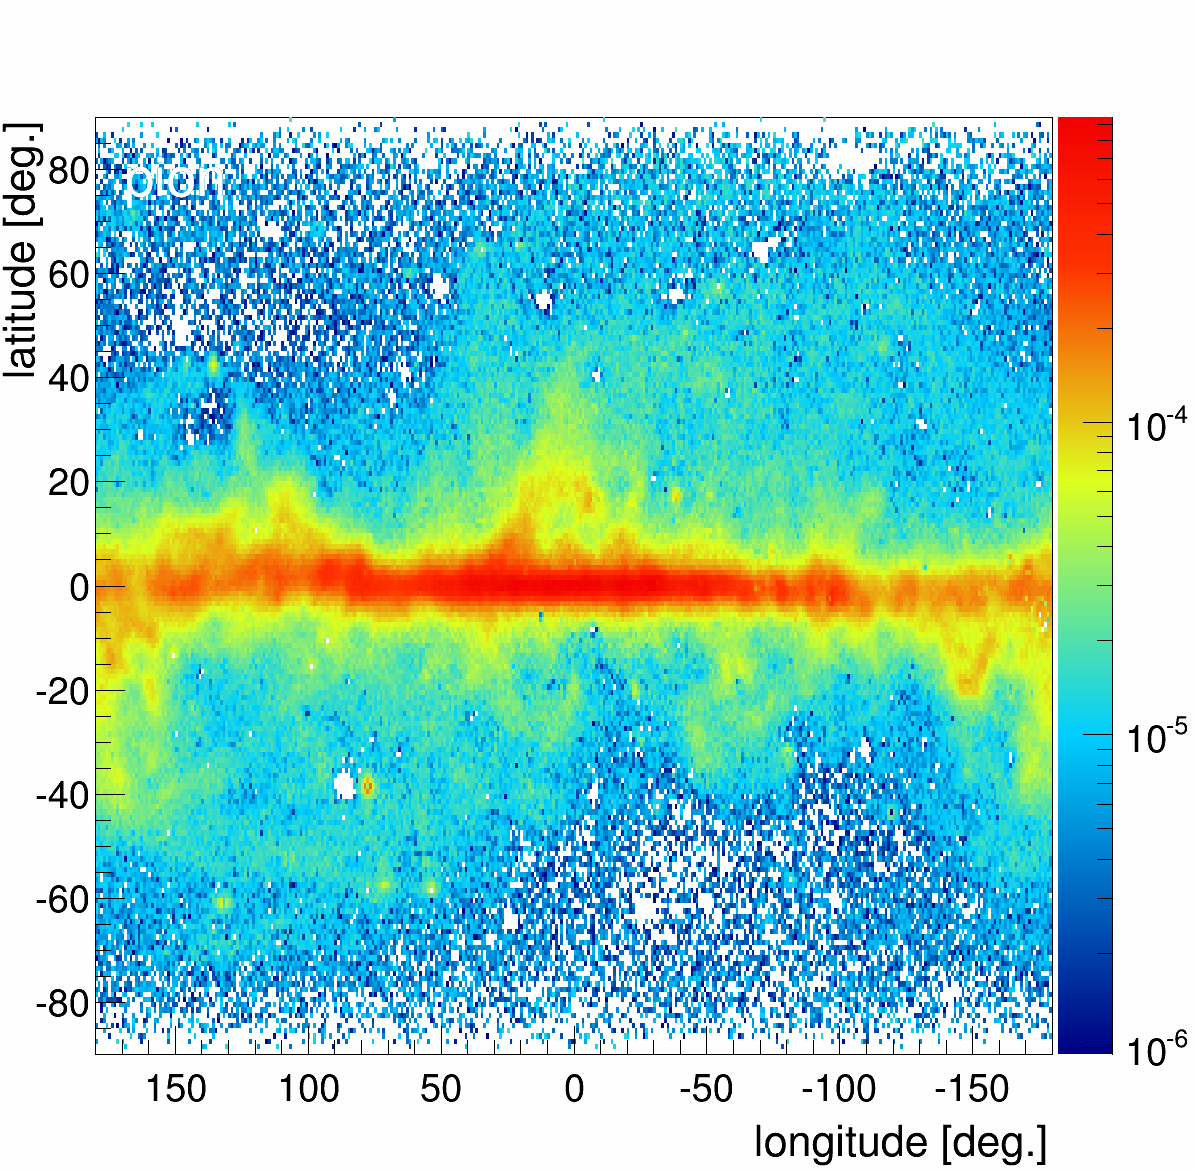
\includegraphics[width=1.\linewidth]{pic/results/SCR_PCR_Integral.png}
  	\subcaption{}
  	\label{app:BKGonly_PCR}
  \end{minipage}
  \hfill
  \begin{minipage}[h]{0.45\textwidth}
  	\centering
	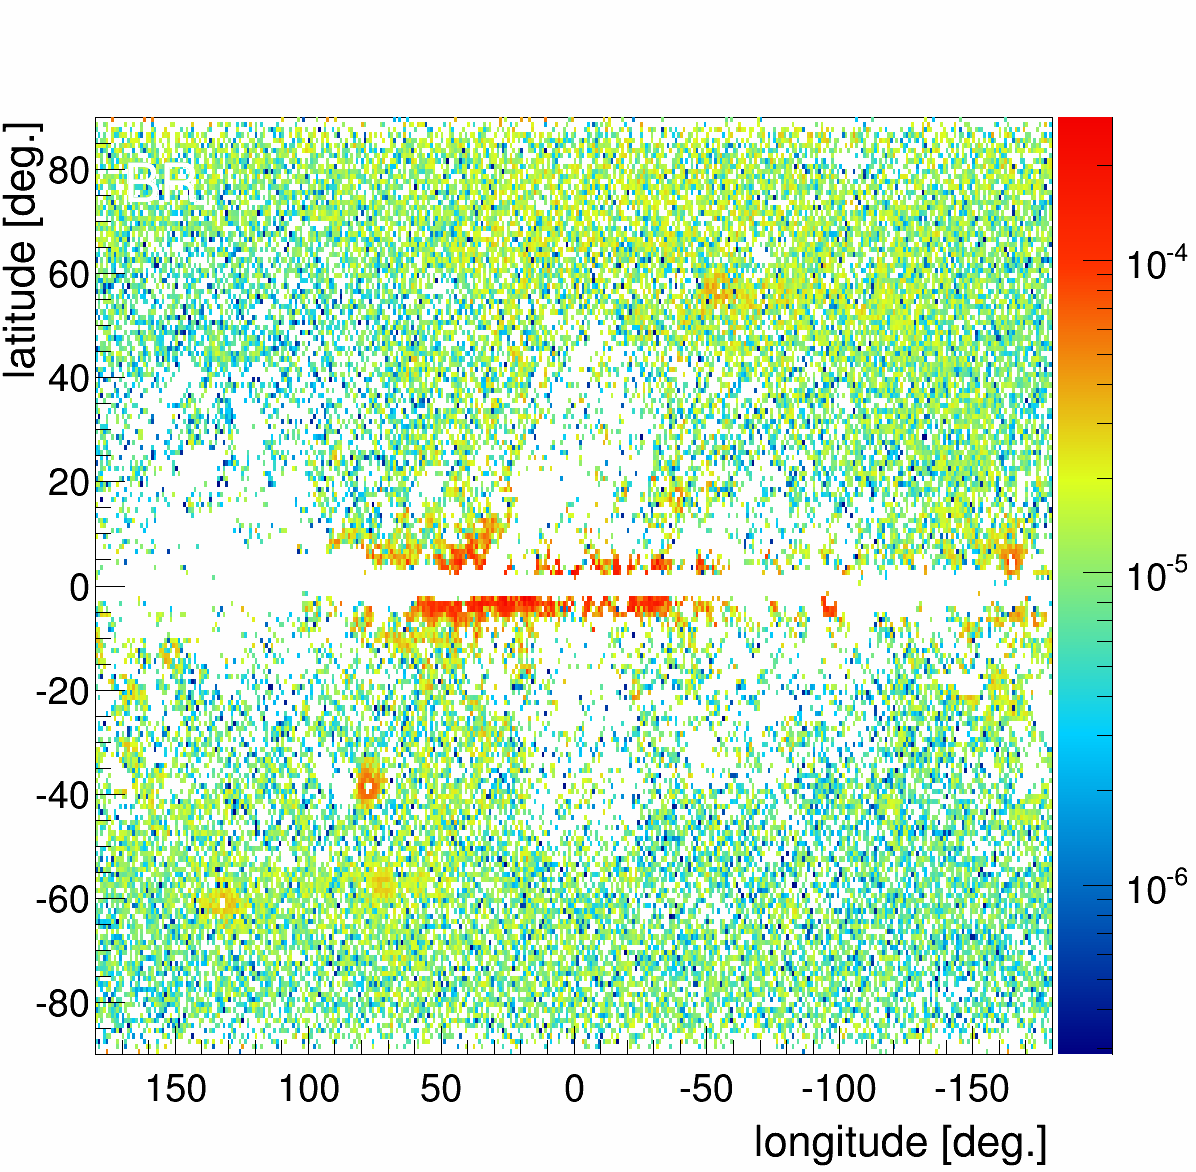
\includegraphics[width=1.\linewidth]{pic/results/SCR_BR_Integral.png}
  	\subcaption{}
  	\label{app:BKGonly_BR}
  \end{minipage}
  \hfill
  \begin{minipage}[h]{0.45\textwidth}
  	\centering
	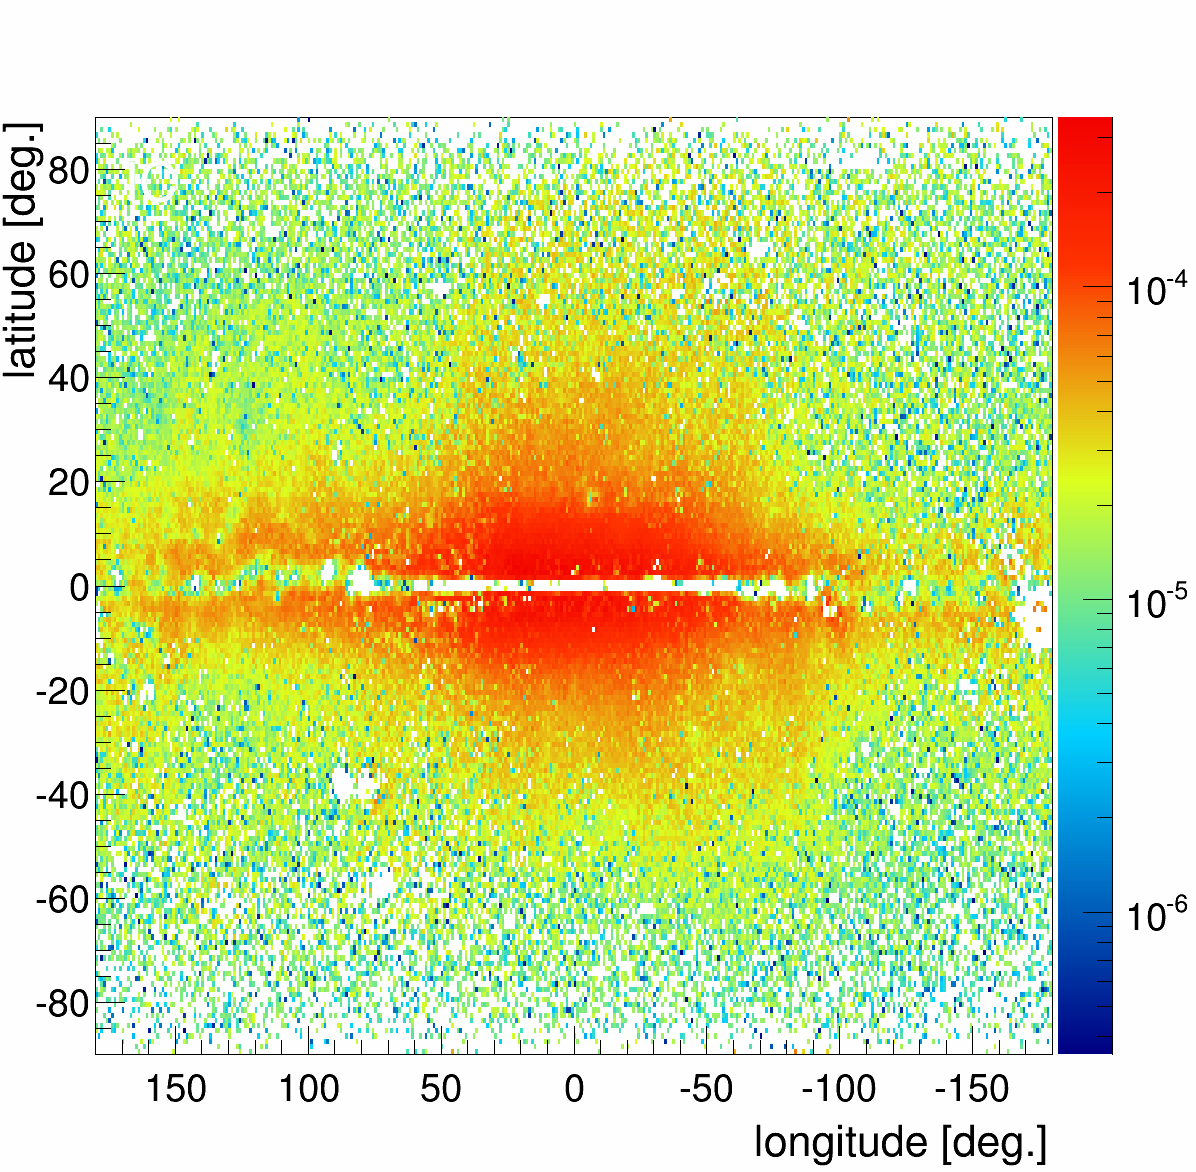
\includegraphics[width=1\linewidth]{pic/results/SCR_IC_Integral.png}
 	\subcaption{}
  	\label{app:BKGonly_IC}
  \end{minipage}
  \hfill
  \begin{minipage}[h]{0.45\textwidth}
  	\centering
	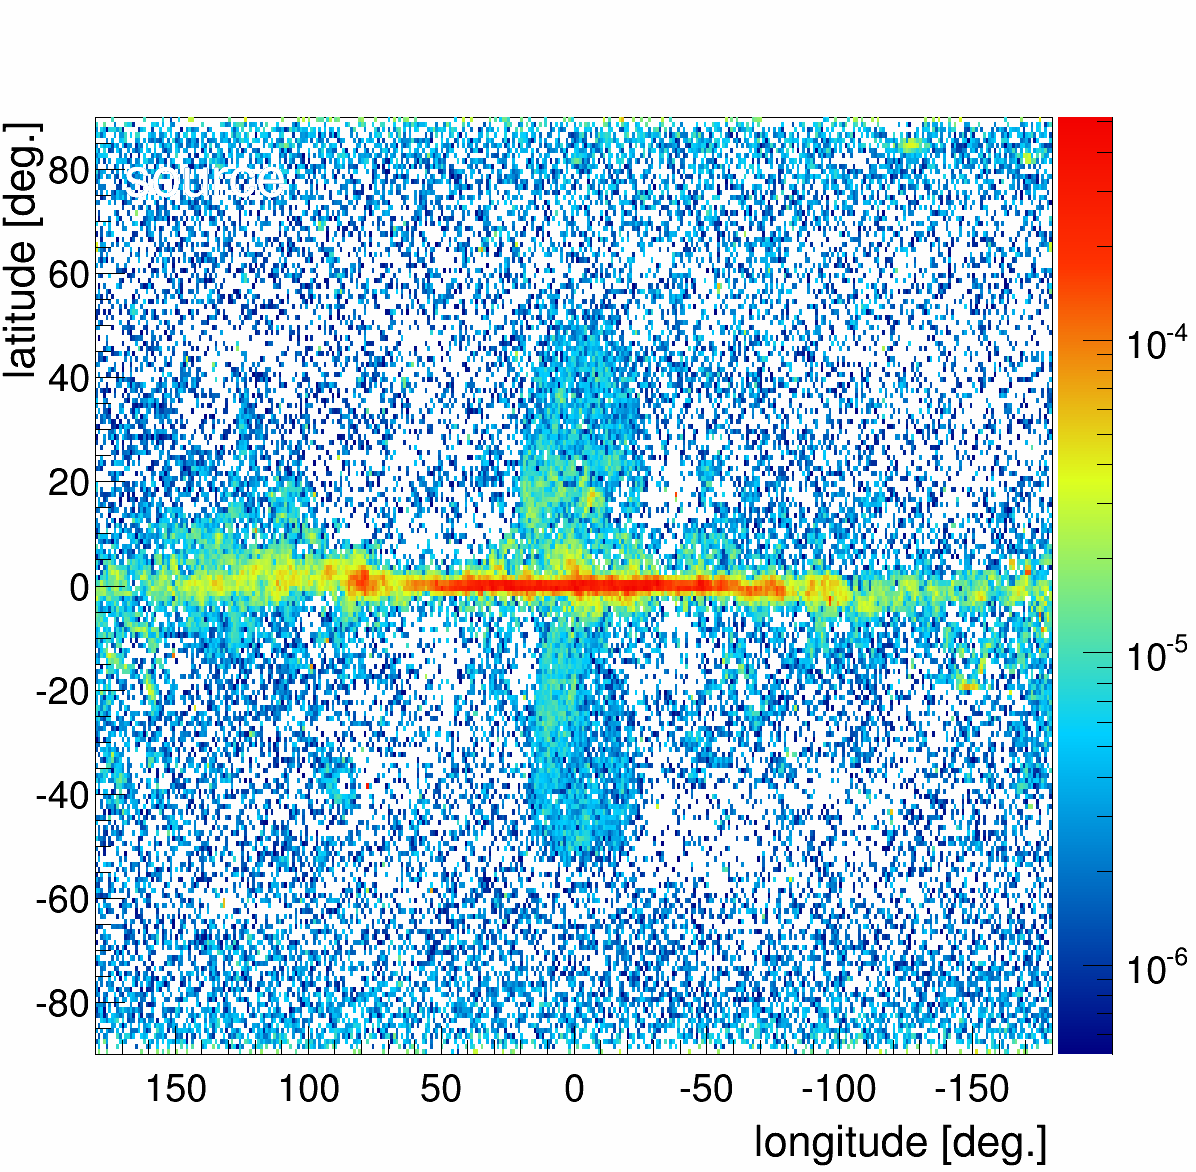
\includegraphics[width=1\linewidth]{pic/results/SCR_SCR_Integral.png}
 	\subcaption{}
  	\label{app:BKGonly_IC}
  \end{minipage}
  \caption[Components flux distribution in the background and source fit]{Components flux distribution in the background and source fit. (a) PCR distribution. (b) BR. (c) IC. (d) SCR.}
  \label{app:SCRonly_fit_distributions}
\end{figure}


\newpage
\begin{figure}[H]
  \centering
  \begin{minipage}[h]{0.45\textwidth}
  	\centering
	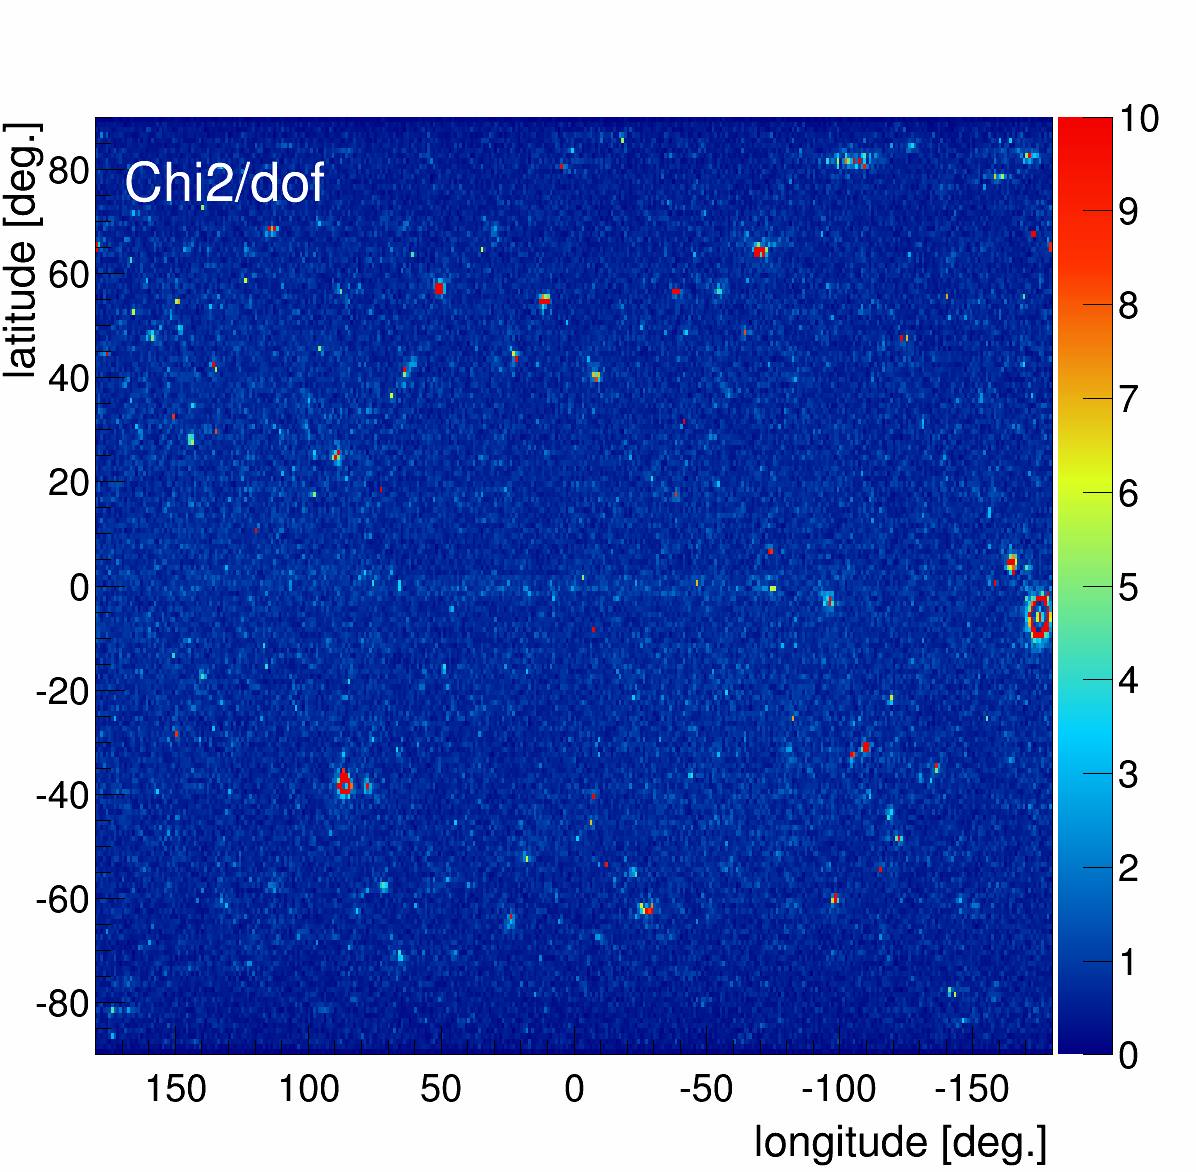
\includegraphics[width=1.\linewidth]{pic/results/MCRonly_fine_chi2_distribution.png}
  	\subcaption{}
  	\label{fig:MCRonly_chi2Distribution}
  \end{minipage}
  \hfill
  \begin{minipage}[h]{0.45\textwidth}
  	\centering
	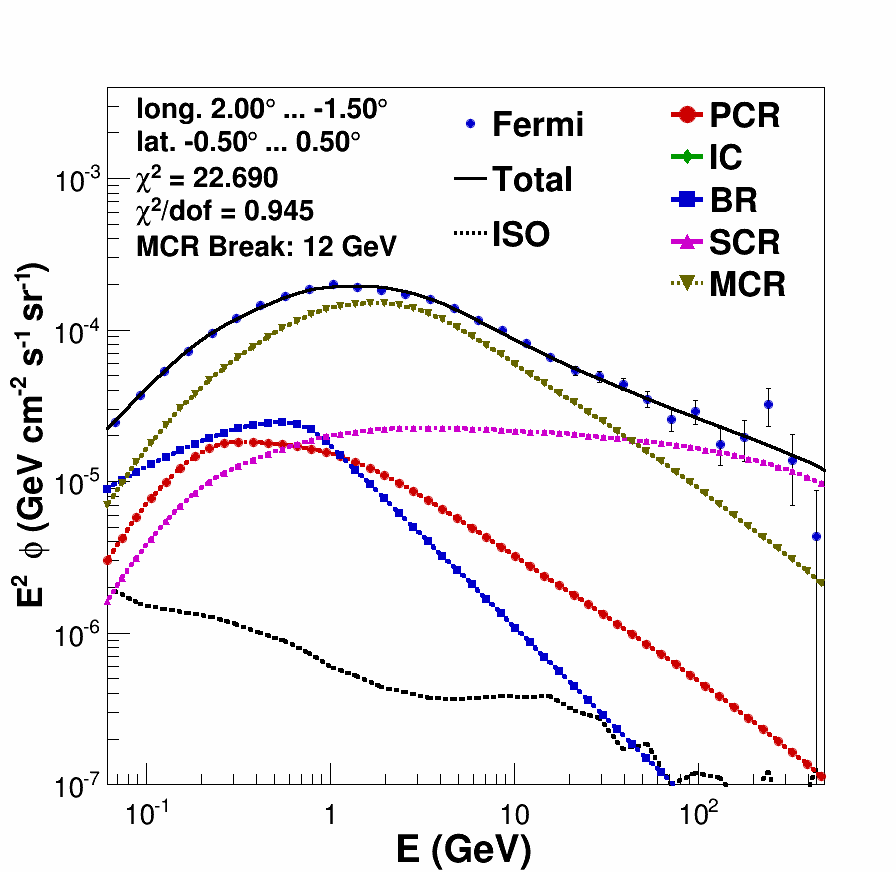
\includegraphics[width=\linewidth]{pic/results/MCRonly_CMZ.png}
	\subcaption{}
  	\label{fig:MCRonly_CMZ}
  \end{minipage}
  \hfill
  \begin{minipage}[h]{0.45\textwidth}
  	\centering
	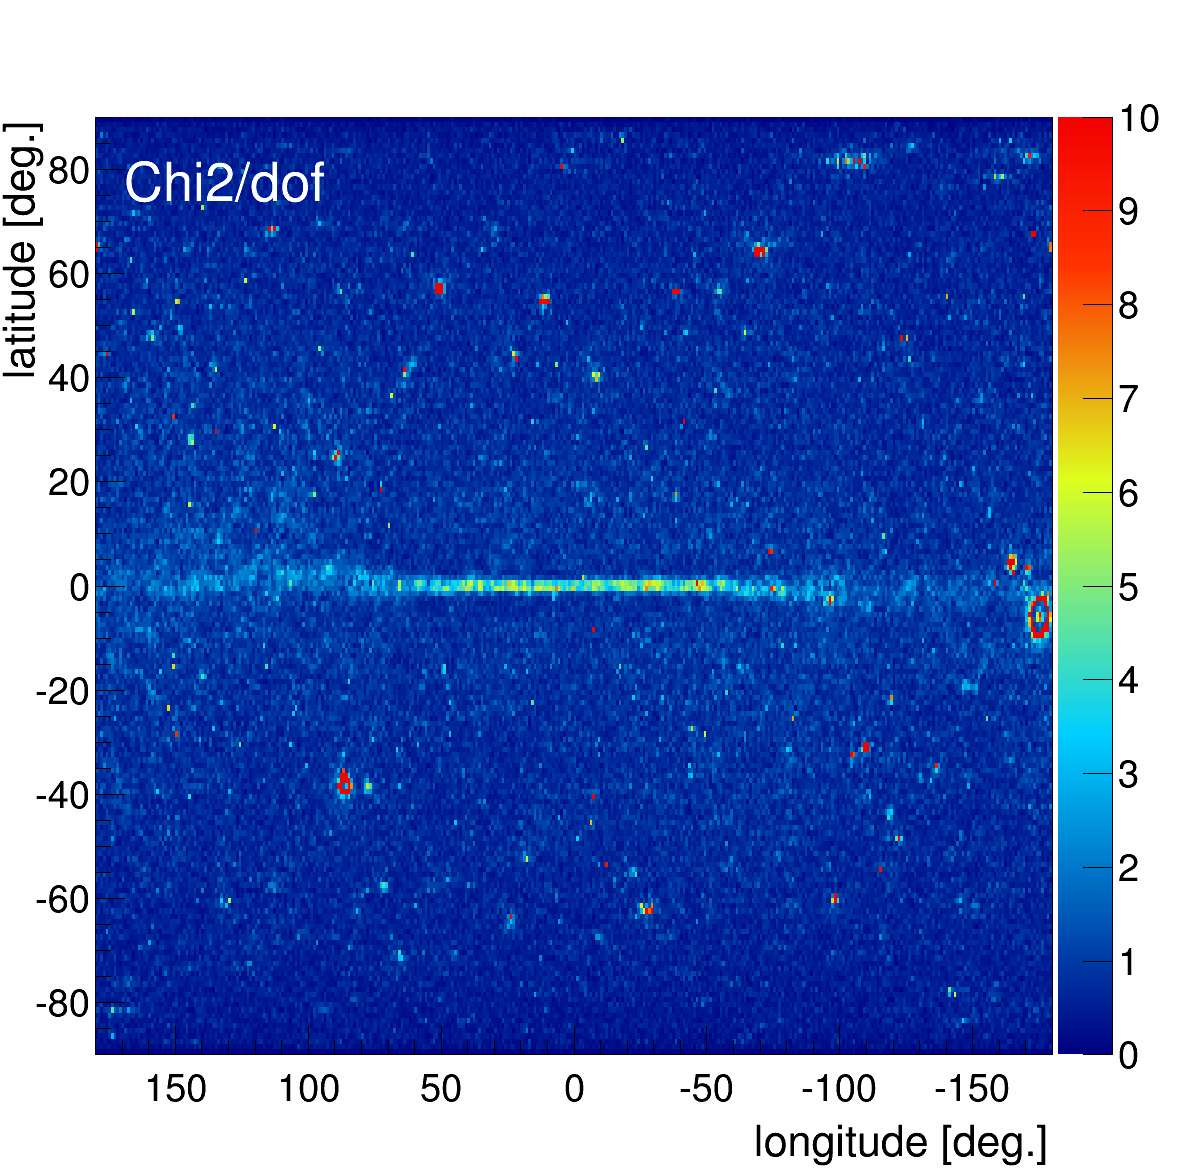
\includegraphics[width=1\linewidth]{pic/results/DMonly_fine_chi2_distribution.png}
  	\subcaption{}
  \label{fig:DMonly_chi2Distribution}
  \end{minipage}
  \hfill
  \begin{minipage}[h]{0.45\textwidth}
  	\centering
	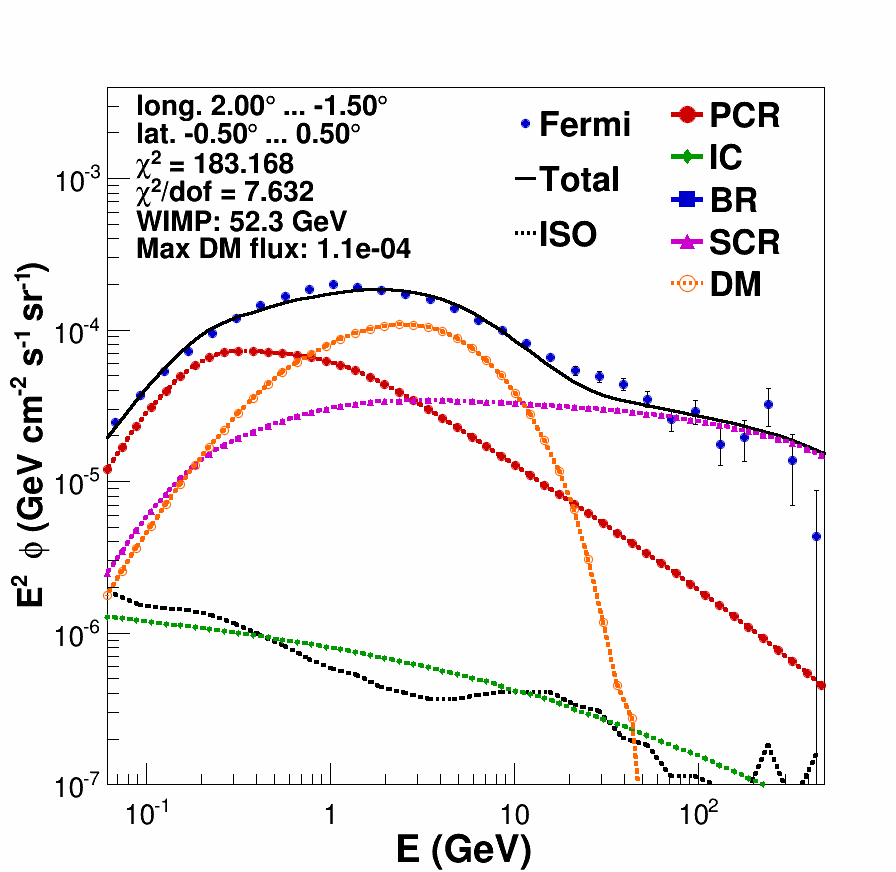
\includegraphics[width=1\linewidth]{pic/results/DMonly_CMZ.png}
  	\subcaption{}
  	\label{fig:DMonly_CMZ}
  \end{minipage}
  \hfill
  \begin{minipage}[h]{0.45\textwidth}
  	\centering
	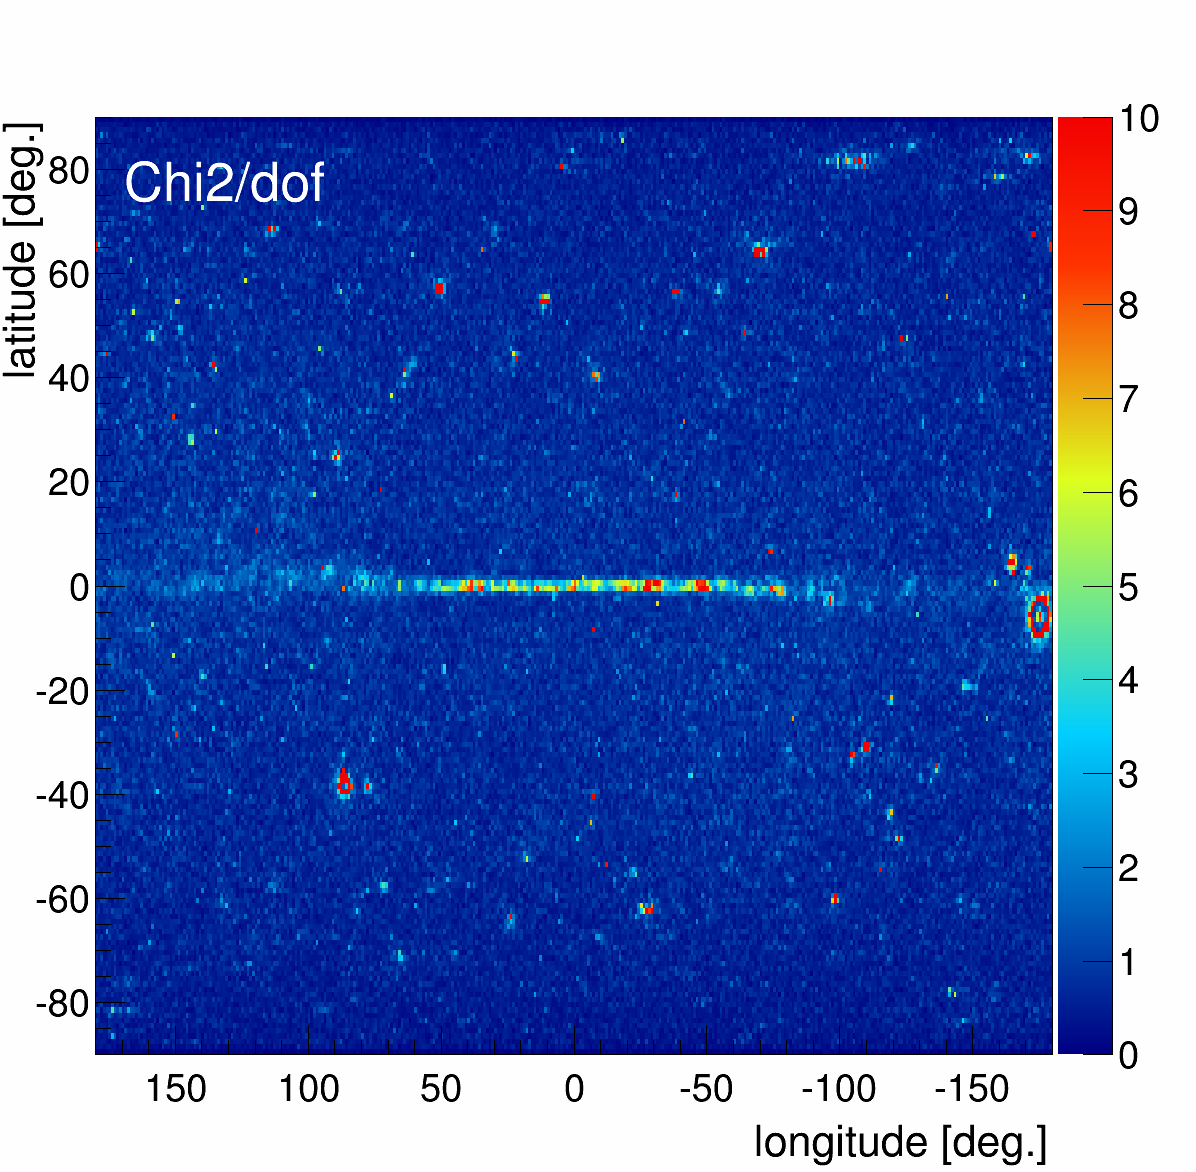
\includegraphics[width=1\linewidth]{./pic/results/MSPonly_fine_chi2_distribution.png}
  	\subcaption{}
  \label{fig:MSPonly_chi2Distribution}
  \end{minipage}
  \hfill
  \begin{minipage}[h]{0.45\textwidth}
  	\centering
	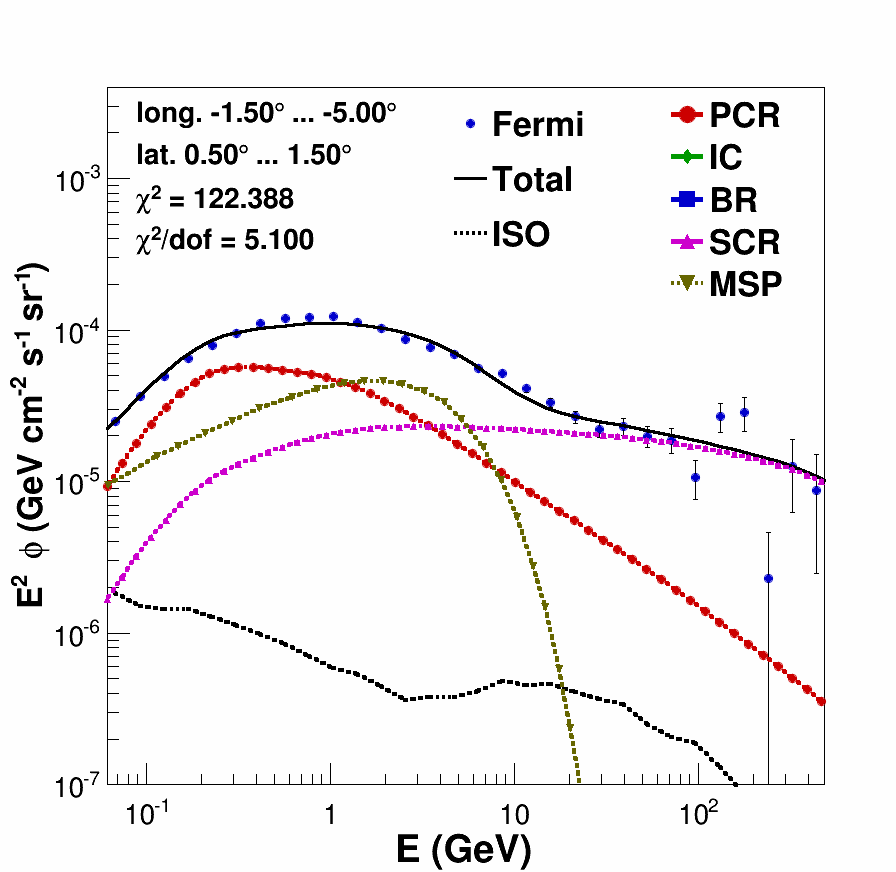
\includegraphics[width=1\linewidth]{pic/results/MSPonly_CMZ.png}
  	\subcaption{}
  	\label{fig:MSP_only_CMZ}
  \end{minipage}
  \caption[$\chi^2$ distributions and CMZ spectra for the MCR, DM and MSP fits.]{Comparison of the $\chi^2$ distributions for the three excess fits (left column) and the CMZ region (right column). MCR (top row), shows a flat $\chi^2$ distribution map, with almost no sign of the disk, and the CMZ is modelled at all energies. DM (middle row) does not fit the disk so well, and the CMZ is not described correctly above 10 GeV. MSP (bottom row) resemble a lot the DM model, with problems in the disk and a poor fit of the CMZ at high energies.}
  \label{fig:Excess_comp_comparison}
\end{figure}

\newpage
\begin{figure}[H]
\centering
  \begin{minipage}[h]{0.7\linewidth}
  	\centering
	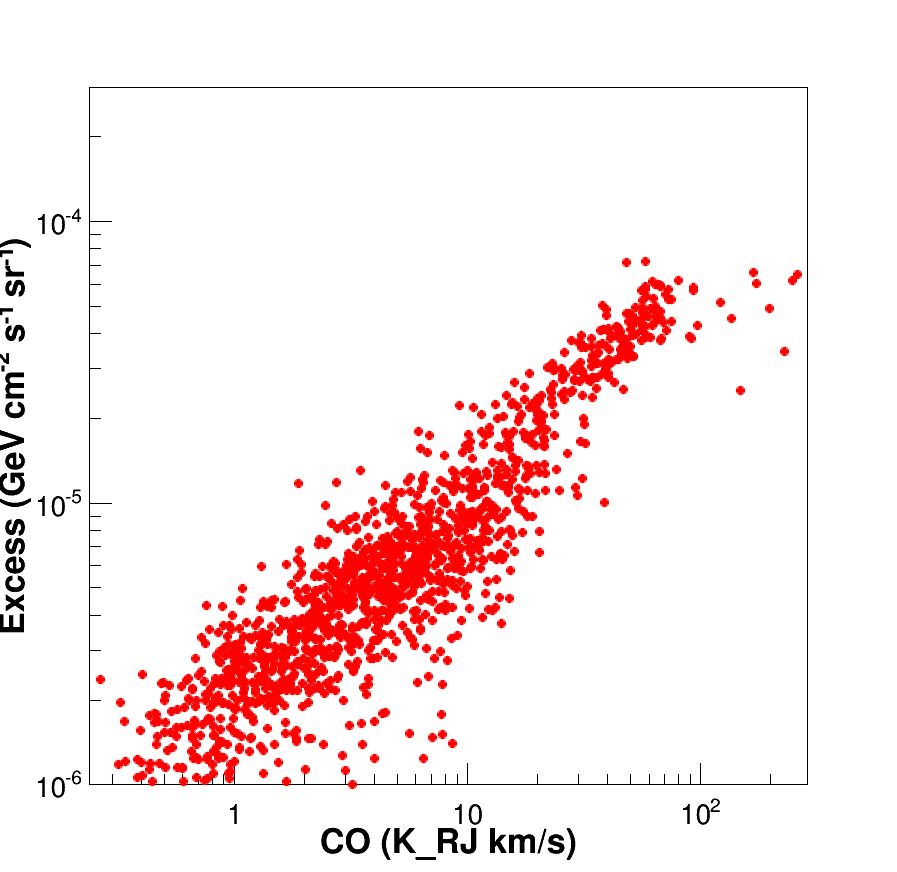
\includegraphics[width=1\linewidth]{./pic/results/COvsDM_2_Spectra.png}
  	\subcaption{}
  \label{fig:DM_CO_correlation}
  \end{minipage}
  \hfill
  \begin{minipage}[h]{0.7\linewidth}
  	\centering
	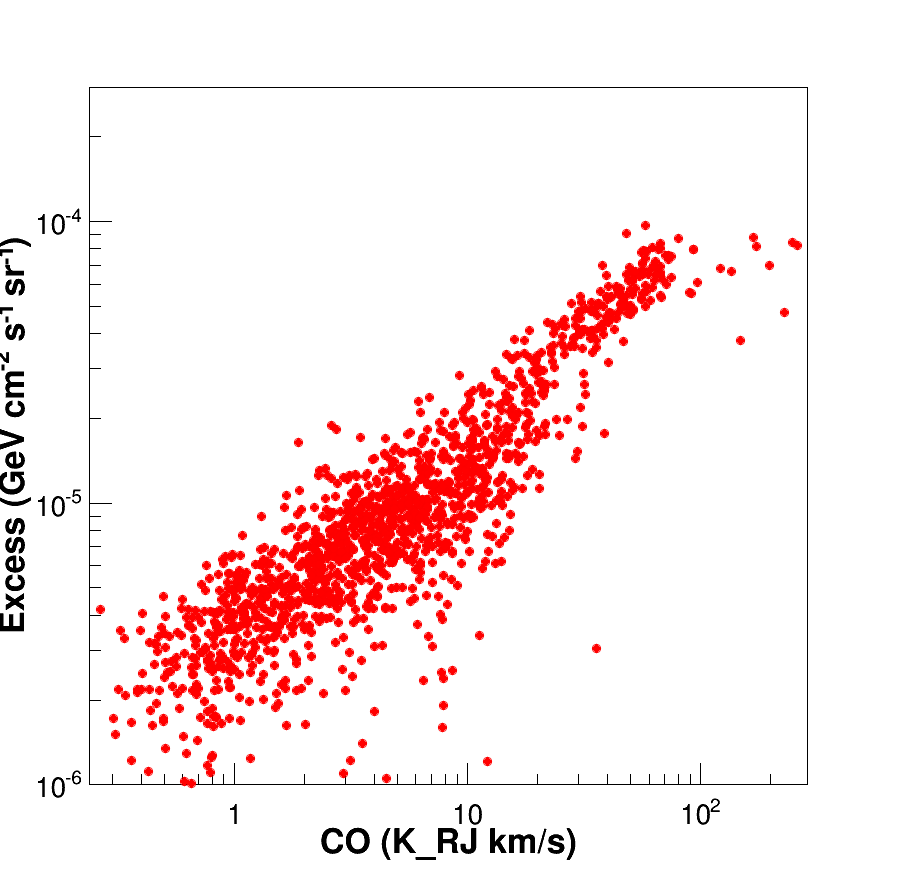
\includegraphics[width=1\linewidth]{pic/results/COvsMSP_2_Spectra.png}
  	\subcaption{}
  	\label{fig:MSP_CO_correlation}
  \end{minipage}
  \caption[Correlation of DM and MSP to CO emission.]{DM (a) and MSP (b) flux plotted against CO flux in every cones of one by one degree below two degrees in latitude. The correlation is clear and directly links the excess component to the galactic MCs.}
  \label{app:DM_MSP_CO_correlation}	 
\end{figure}



\newpage
\section{To go further: How to improve the model}
\label{app:PCR+MCR_distribution}
\begin{figure}[H]
  \centering
  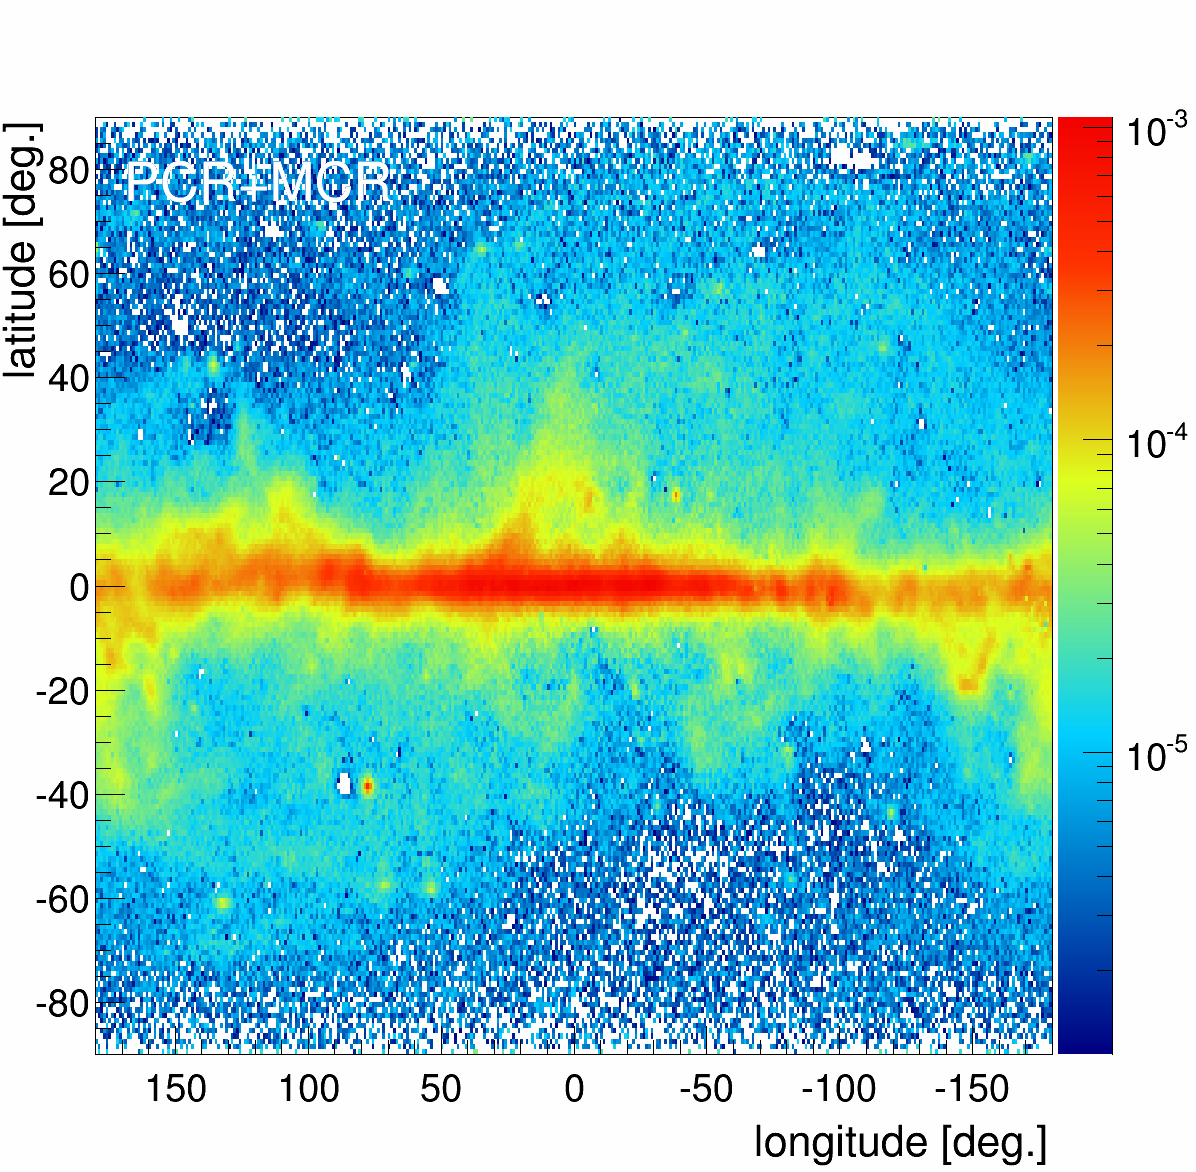
\includegraphics[width=\linewidth]{pic/discussion/MCRonly_fine_PCR+MCR_integral_distribution.png}	 
  \caption[Skymap of the PCR and MCR sum.]{Sum of PCR and MCR spatial distribution for the MCR fit.}
  \label{app:PCR+MCR_integral_distribution}	 
\end{figure}



%\begin{table}[]
%\centering
%\caption{My caption}
%\label{my-label}
%\begin{tabular}{p{\linewidth}}

%\end{tabular}
%\end{table}
